\appendix

\section{Notation and derivations}
\label{app:derivations}

\subsection{Notation and estimand fine print}
\label{app:notation}

\paragraph{Arm labels versus route subscripts.}
One notational convention holds throughout. Arm labels ($\src$,
$\reenc$, $\dem$) mark \emph{whose} gradient, latent, or Jacobian an
object is; the subscript on every route-level scalar is the
\emph{route}, written in full ($d_{e_0 \to e}$) where several sources
appear, and abbreviated to the target edge alone wherever the source
edge is fixed by context, as it is in almost every measured
statement; the abbreviation is an edge value, never an arm label, so
it always instantiates numerically ($d_e$, $\Phi_{1120}$,
$\mathrm{Resid}_{768}$). The
control's distance $d_{\reenc}$ (Eq.~\ref{eq:gapdef} with
$\bar g_{\reenc}$ in place of $\bar g_{\dem}$) is the one exception that
carries an arm label: the control changes no grid and has no target
edge. Each table states which object it reports, $d_e$ or the excess
$\gap_e$.

\paragraph{The two aggregations.}
In a batched training scenario Eq.~\ref{eq:gapdef} admits two
aggregations over a probe set: per-example (cosine per image, then
mean; the object every map in the body reports) or batch-aggregate
(gradients summed over the batch before the cosine; the object SGD
actually follows). These are different estimands, since the
aggregation operator is part of the estimand, and no coefficient
fitted on one is guaranteed to transfer to the other. At second order the two
are related by a batch-size decomposition: writing each image's
demotion-induced gradient disagreement as a coherent mean $b$ plus a
zero-mean idiosyncratic deviation with covariance $\Sigma_\eta$, the
batch-aggregate distance at batch size $B$ is
\begin{equation*}
\mathbb{E}[d_B] \;\approx\;
\frac{\|P^{\perp} b\|^2}{2\|\mu\|^2}
\;+\;
\frac{\mathrm{tr}\!\big(P^{\perp} \Sigma_\eta P^{\perp}\big)}{2B\|\mu\|^2},
\end{equation*}
with $\mu$ the mean source gradient and $P^{\perp}$ the projector off
$\hat\mu$: an intercept (the coherent share, which never averages
out) plus a $1/B$ term. Monotone improvement with $B$ is not
automatic, since it would require an iid zero-mean disagreement model
we have not verified, but where we have measured the batch object it
is the more forgiving of the two: pooled-arm probes at pool size $4$
collapse the $1024{\to}896$ excess to ${\approx}\,0$ at every bin
$\sigma \ge 0.625$ and the $1024{\to}768$ excess at
$\sigma \ge 0.875$ (\S\ref{sec:map}), the $1/B$ term dominating
there. What the collapse does not bound is the intercept, exactly the
coherent drift that the intercept-plus-$1/B$ fit across pool sizes
(\S\ref{sec:map}) is designated to bound.

\subsection{Derivation of the branch decomposition
(Eq.~\ref{eq:branches})}
\label{app:branches}

Fix a query (image, caption), a $\sigma$, and an arm $a$. Per draw
$\epsilon$, the adapter gradient of the $\tfrac12$-scaled loss is the
product $g_a(\epsilon) = J_a(\epsilon)^{\!\top} r_a(\epsilon)$ of
\S\ref{sec:ouraccount}. Split each factor into its noise mean and
fluctuation, $J_a = \bar J_a + \tilde J_a$ and
$r_a = \bar r_a + \tilde r_a$ with
$\mathbb{E}_\epsilon[\tilde J_a] = 0$ and
$\mathbb{E}_\epsilon[\tilde r_a] = 0$; the population mean gradient of
arm $a$ is then
\begin{equation}
\bar g_a \;=\; \mathbb{E}_\epsilon\!\big[J_a^{\!\top} r_a\big]
\;=\; \bar J_a^{\!\top} \bar r_a
\;+\; \mathbb{E}_\epsilon\!\big[\tilde J_a^{\!\top} \tilde r_a\big].
\label{eq:appmean}
\end{equation}
Write the demoted arm's mean factors as native plus a perturbation,
$\bar J_{\dem} = \bar J + \Delta J$ and $\bar r_{\dem} = \bar r + \Delta \bar r$
(bars without an arm subscript denote the native arm). Subtracting
Eq.~\ref{eq:appmean} across arms and expanding the product,
\begin{equation}
\delta g \;=\; \bar g_{\dem} - \bar g_{\src}
\;=\;
\underbrace{\bar J^{\!\top} \Delta\bar r}_{\text{data branch }B_e}
\;+\;
\underbrace{\Delta J^{\!\top}\, \bar r}_{\text{graph branch }C_e}
\;+\;
\underbrace{\Delta J^{\!\top} \Delta\bar r
\;+\;
\mathbb{E}_\epsilon\!\big[\tilde J_{\dem}^{\!\top}\tilde r_{\dem}\big]
- \mathbb{E}_\epsilon\!\big[\tilde J_{\src}^{\!\top}
\tilde r_{\src}\big]}_{\text{remainder }R_e}.
\label{eq:appbranches}
\end{equation}
This is an exact identity: no linearization is involved.
``First-order'' in the main text refers only to the content of $R_e$:
it collects every term that is a product of two perturbations
($\Delta J^{\!\top} \Delta\bar r$) or a difference of noise-covariance
terms (the last two). Eq.~\ref{eq:branches} is
Eq.~\ref{eq:appbranches} with the covariance difference abbreviated
into its ellipsis.

One remark delimits the identity's literal scope. When the two arms
share a grid (as for the re-encoding control), every operation above is
literal. Across grids, $J_{\src}$ and $J_{\dem}$ act on different
token counts, so the differences $\Delta J$ and $\Delta \bar r$ require
a fixed identification of the two output spaces (e.g.\ spectral
zero-padding of the coarse grid onto the fine grid's bands); any such
identification changes the split between $B_e$, $C_e$, and $R_e$ but
not their sum $\delta g$, which lives in the shared adapter-parameter
space regardless. This is why the main text defines the branches
\emph{operationally} (as the two independent perturbation directions
in adapter-parameter space, isolated by the designated probes of
\S\ref{sec:ourscored}) and treats Eq.~\ref{eq:branches} as fixing what
each branch collects rather than as a computable matrix formula.

\subsection{The mean residual as a posterior operator}
\label{app:posterior}

This appendix derives the posterior form of the fixed-image mean
residual, the exact split of the measured object into intrinsic
posterior bias plus model approximation error, and the Gaussian
closure referenced in \S\ref{sec:reduction}. Fix a caption $c$ and
grid $e$, write $a = 1 - \sigma$, and let $x \sim p_e(\cdot \mid c)$
be the grid-$e$ clean latent, $z_\sigma = a x + \sigma \epsilon$ with
$\epsilon \sim \mathcal{N}(0, I)$.

\paragraph{Bayes field and fixed-image residual.}
For the squared objective the population-optimal field is the
conditional mean of the target
$v = \epsilon - x = (z_\sigma - x)/\sigma$:
\begin{equation}
v_e^{*}(z, \sigma, c)
\;=\; \mathbb{E}[v \mid z_\sigma = z,\, c]
\;=\; \frac{z - m_e(z, c)}{\sigma},
\qquad
m_e(z, c) := \mathbb{E}[x \mid z_\sigma = z,\, c].
\label{eq:appbayesfield}
\end{equation}
Averaging over noise at fixed image
($\mathbb{E}_\epsilon[\epsilon] = 0$,
$\mathbb{E}_\epsilon[z_\sigma] = a x$) gives the posterior form
used in \S\ref{sec:reduction}:
\begin{equation}
\bar r_e^{*}(\sigma; x)
\;=\; \mathbb{E}_\epsilon\big[v_e^{*}(a x + \sigma \epsilon, \sigma, c)
      - (\epsilon - x)\big]
\;=\; \frac{x - \mathbb{E}_{z_\sigma \mid x}\big[m_e(z_\sigma,
      c)\big]}{\sigma}.
\label{eq:appposterior}
\end{equation}
With $p_{\sigma,e}(z \mid c)$ the noised marginal, Tweedie's identity
for the linear interpolant reads
$m_e(z, c) = \big(z + \sigma^2 \nabla_z \log p_{\sigma,e}(z \mid
c)\big)/a$ for $\sigma < 1$, so equivalently
\begin{equation}
\bar r_e^{*}(\sigma; x)
\;=\; -\frac{\sigma}{1 - \sigma}\,
\mathbb{E}_{z_\sigma \mid x}\big[\nabla_z \log
p_{\sigma,e}(z_\sigma \mid c)\big],
\label{eq:appscore}
\end{equation}
which makes the missing ingredient explicit: the numerical curve
requires the grid- and caption-conditional smoothed score, i.e.\ a
model of $p_e(x \mid c)$. At $\sigma = 1$, where $z = \epsilon$ is
independent of $x$, $m_e(z, c) \to \mathbb{E}[x \mid c]$ and
$\bar r_e^{*}(1; x) = x - \mathbb{E}[x \mid c]$. With $A_e$ the
alignment operator that places the source-grid residual on the demoted
grid (\S\ref{sec:instrument}), the Bayes-level cross-grid mismatch is
$\Delta \bar r_e^{*}(\sigma; x) = \bar
r_{\dem}^{*}(\sigma; x_{\dem}) - A_e \bar r_{\src}^{*}(\sigma;
x_{\src})$.

\paragraph{What the instrument measures.}
MSE optimality gives $\mathbb{E}[v^{*} - v \mid z, c] = 0$ and hence a
zero residual after a \emph{joint} average over $(x, \epsilon)$; it
does not zero the fixed-image average
$\mathbb{E}_\epsilon[v^{*} - v \mid x, c]$, which is
Eq.~\ref{eq:appposterior} and generally nonzero. Writing the trained
network as $\hat v_{\theta,e} = v_e^{*} + q_{\theta,e}$, the probe's
per-image object splits exactly as
\begin{equation}
\bar r_{\theta,e}(\sigma; x)
\;=\; \bar r_e^{*}(\sigma; x)
\;+\; \mathbb{E}_{z_\sigma \mid x}\big[q_{\theta,e}(z_\sigma, \sigma,
c)\big]:
\label{eq:appsplit}
\end{equation}
intrinsic posterior reconstruction bias, derivable in principle from
$p_e(x \mid c)$, plus genuinely model-specific approximation error.
The measured $\|\Delta \bar r(\sigma)\|$ therefore has definite
theoretical status, as an empirical closure of
Eq.~\ref{eq:appposterior}, but is not a pure model-error
difference, and no claim in the paper requires it to be one: the
two-term account consumes the measured curve as-is
(assumption~(iv)), and the trained-model residual is in any case the
exact $r$-factor that the LoRA gradient $g = J^{\!\top} r$ is built
from.

\paragraph{Gaussian closure.}
The cheapest nontrivial closure is a full Gaussian model
$x \mid c \sim \mathcal{N}(\mu_e, C_e)$ per grid. With
$Q_e(\sigma) = a^2 C_e + \sigma^2 I$, the posterior mean is linear,
$m_e(z, c) = \mu_e + a C_e Q_e^{-1}(z - a \mu_e)$, and substituting
into Eq.~\ref{eq:appposterior} collapses (via
$I - a^2 C_e Q_e^{-1} = \sigma^2 Q_e^{-1}$) to
\begin{equation}
\bar r_e^{*}(\sigma; x) \;=\; \sigma\, Q_e(\sigma)^{-1} (x - \mu_e).
\label{eq:appgaussian}
\end{equation}
For paired source and demoted latents with covariance blocks
$C_{ss}, C_{dd}, C_{ds}$ and $L_s = \sigma Q_s^{-1}$,
$L_d = \sigma Q_d^{-1}$, the image-population mean squared mismatch is
\begin{equation}
\mathbb{E}\big\|\Delta \bar r_e^{*}\big\|^2
= \operatorname{tr}\!\big(L_d C_{dd} L_d^{\!\top}\big)
+ \operatorname{tr}\!\big(A_e L_s C_{ss} L_s^{\!\top}
  A_e^{\!\top}\big)
- 2 \operatorname{tr}\!\big(L_d C_{ds} L_s^{\!\top}
  A_e^{\!\top}\big),
\label{eq:apptrace}
\end{equation}
a $\sigma$-curve computable from paired \emph{clean latents only},
with the source--demote cross-covariance $C_{ds}$ load-bearing. A
\emph{diagonal Fourier} $C_e$ makes Eq.~\ref{eq:appgaussian} the
per-band Wiener shrinkage of \S\ref{sec:spectral}, confining the
mismatch to the destroyed band and ordering it by destroyed-band
energy: the residual-level prediction that route-uniformity
falsifies (\S\ref{sec:ourscored}). We tested whether any structured
second-order closure suffices, entirely on stored paired clean
latents (no denoiser forward): three nested covariance models
(diagonal spectral; $+$\,within-band channel blocks;
$+$\,octave-pair cross-band coupling), fitted on held-out-from-probe
images and scored on the probe set against the measured curves. All
three reproduce the curve's monotone $\sigma$-shape (Pearson
$0.94$--$0.97$), its route-uniformity, the near-zero re-encoding
control, and the $\sigma{=}1$ endpoint, but over-predict the
low-$\sigma$ amplitude by ${\sim}40\%$, failing a pre-registered
RMSE bar. Second-order data-only structure therefore recovers the
shape but not the level, and the essential missing ingredients are
the ones the identity names: caption-conditioning (the closure is
caption-marginal), non-Gaussian posterior structure, and the
$q_{\theta}$ term of Eq.~\ref{eq:appsplit}. The paper therefore
retains the measured $\|\Delta \bar r(\sigma)\|$ as its minimal
honest closure. A theory--instrument comparison must also reproduce
the instrument's estimand, the split-half-corrected \emph{relative}
$L_2$ distance of \S\ref{sec:instrument}, i.e.\
$\sqrt{\mathbb{E}\|\bar r_d - A_e \bar r_s\|^2}$ normalized by the
mean of the two arms' root-mean-square norms, rather than a raw
mismatch norm.

\subsection{The angular reduction: exact form and four-term expansion}
\label{app:geometry}

This appendix states and derives the two angular forms summarized in
\S\ref{sec:reduction}. Both follow from Eq.~\ref{eq:gapdef} and the
split of $\delta g$ by the native direction; no property of demotion
enters. Write $g = \bar g_{\src}$, $G = \|g\|$, $\hat g = g/G$, and
$u^{\perp} = u - (\hat g^{\!\top}u)\,\hat g$; decompose
$\delta g = G\,\kappa_\parallel\, \hat g + \delta g^{\perp}$ with
$\kappa_\parallel = \hat g^{\!\top}\delta g / G$ and
$\kappa_\perp = \|\delta g^{\perp}\| / G$.

\paragraph{The exact form.} The two components are orthogonal, so
$\|g + \delta g\|^2 = G^2 (1+\kappa_\parallel)^2 + G^2 \kappa_\perp^2$
and
\begin{equation}
\cos\big(g,\, g + \delta g\big)
\;=\; \frac{\hat g^{\!\top}(g + \delta g)}{\|g + \delta g\|}
\;=\; \frac{1 + \kappa_\parallel}
{\sqrt{(1+\kappa_\parallel)^2 + \kappa_\perp^2}}
\;=\; \frac{1}{\sqrt{1 + \kappa_{\mathrm{eff}}^2}}\,,
\qquad
\kappa_{\mathrm{eff}} = \frac{\kappa_\perp}{1 + \kappa_\parallel}\,,
\label{eq:appexact}
\end{equation}
valid whenever $1 + \kappa_\parallel > 0$ (the perturbation does not
reverse the gradient direction). The gap of Eq.~\ref{eq:gapdef} is
therefore, \emph{exactly},
\begin{equation}
d_e \;=\; 1 - \frac{1}{\sqrt{1 + \kappa_{\mathrm{eff}}^2}}\,,
\label{eq:exact}
\end{equation}
the exact angular link of \S\ref{sec:reduction}. Since
$1 - \cos(\hat g_1, \hat g_2) = \tfrac12 \|\hat g_1 - \hat g_2\|^2$
for unit vectors, starting from either expression in
Eq.~\ref{eq:gapdef} lands on the same result.

\paragraph{The quadratic limit.} For small perturbations,
$1 - (1 + \kappa_{\mathrm{eff}}^2)^{-1/2}
= \tfrac12 \kappa_{\mathrm{eff}}^2 + O(\kappa_{\mathrm{eff}}^4)$ and
$\kappa_{\mathrm{eff}}^2 = \kappa_\perp^2\big(1 - 2\kappa_\parallel
+ O(\kappa_\parallel^2)\big)$, so
\begin{equation}
d_e \;=\; \frac{\|\delta g^{\perp}\|^2}{2 G^2}
\;+\; \underbrace{O(\kappa_\perp^2 \kappa_\parallel)
+ O(\kappa_\perp^4)}_{\text{beyond-quadratic}}.
\label{eq:appquad}
\end{equation}

\paragraph{The four-term expansion.} Substituting
$\delta g = B_e + C_e + R_e$ (Eq.~\ref{eq:appbranches}) into the leading
term and expanding the square,
\begin{equation*}
\|\delta g^{\perp}\|^2
= \|B_e^{\perp}\|^2 + \|C_e^{\perp}\|^2
+ 2\,\langle B_e^{\perp},\, C_e^{\perp}\rangle
+ \Big(2\,\langle (B_e{+}C_e)^{\perp},\, R_e^{\perp}\rangle
+ \|R_e^{\perp}\|^2\Big),
\end{equation*}
whose first three terms, divided by $2G^2$, define the data share, the
graph share, and the projected interaction:
\begin{equation}
d_e(\sigma) \;\approx\;
\underbrace{\frac{\big\|B_e^{\perp}\big\|^2}{2\,\|\bar g_{\src}\|^2}}_{\text{data share }S_e}
\;+\;
\underbrace{\frac{\big\|C_e^{\perp}\big\|^2}{2\,\|\bar g_{\src}\|^2}}_{\text{graph share }\Phi_e}
\;+\;
\underbrace{\frac{\big\langle B_e^{\perp},\, C_e^{\perp}\big\rangle}{\|\bar g_{\src}\|^2}}_{\text{projected interaction }I_e}
\;+\; R'_e,
\label{eq:fourterm}
\end{equation}
the four-term expansion of \S\ref{sec:reduction}. The remainder
$R'_e$ has an exact content: the
$R_e$-bearing terms above, the beyond-quadratic terms of
Eq.~\ref{eq:appquad}, and the parallel-component correction, each
suppressed by an extra power of perturbation size relative to the
retained terms.

\paragraph{From the four-term form to the excess.} The reported object
is the excess over the control. The $\reenc$ arm changes no grid, so
$\Delta J_{\reenc} = 0$, and both control terms built from it vanish
identically: its graph share $\Phi_{\reenc}$ and its projected
interaction $I_{\reenc}$ each carry a factor
$(\Delta J_{\reenc}^{\!\top}\bar r)^{\perp} = 0$. Writing
Eq.~\ref{eq:fourterm} for each arm and subtracting term by term,
\begin{align*}
\gap_e(\sigma)
\;&=\; d_e(\sigma) \;-\; d_{\reenc}(\sigma)\\
&\approx\;
\big(S_e - S_{\reenc}\big) \;+\; \big(\Phi_e - \Phi_{\reenc}\big)
\;+\; \big(I_e - I_{\reenc}\big) \;+\; \big(R'_e - R'_{\reenc}\big)
&&\text{Eq.~\ref{eq:fourterm}, each arm}\\
&=\;
\big(S_e - S_{\reenc}\big) \;+\; \Phi_e \;+\; I_e
\;+\; \big(R'_e - R'_{\reenc}\big),
&&\Phi_{\reenc} = I_{\reenc} = 0
\end{align*}
so the control collapses to
$d_{\reenc} \approx S_{\reenc} + R'_{\reenc}$, with $S_{\reenc}$ the
re-encode share (measured ${\approx}\,0$ where probed: the control row
of Table~\ref{tab:floor}). The subtraction cancels only the re-encode
component of the data share (up to a cross term suppressed by
$\sqrt{S_{\reenc}}$, bounded by the control's near-zero reading), so
$\|\Delta\bar r\|$ is read net of re-encode; the graph share and the
interaction pass through untouched, since the control has nothing to
cancel them with.

\paragraph{The drop bounds.} Both discarded terms obey exact bounds in
the retained shares (Cauchy--Schwarz on the expansion above),
\begin{equation}
|I_e| \;\le\; 2\sqrt{S_e\,\Phi_e}\,,
\qquad
\big|R'_e\big| \;\le\; 2\sqrt{\big(S_e + \Phi_e + I_e\big)\,\rho_e}
\;+\; \rho_e
\;+\; O\big(\kappa_\perp^2\kappa_\parallel,\; \kappa_\perp^4\big),
\label{eq:dropbounds}
\end{equation}
with $\rho_e = \|R_e^{\perp}\|^2 / (2\|\bar g_{\src}\|^2)$ the
remainder branch's own share. The first says the interaction can never
exceed the retained sum ($2\sqrt{S_e\Phi_e} \le S_e + \Phi_e$) and is
automatically negligible wherever one share dominates the other, so
assumption (ii) carries independent content only near share
crossover, which is exactly where Appendix~\ref{sec:headtohead} finds
it failing. The second says the first-order part of the remainder
enters at half power, one factor of $\sqrt{\rho_e}$ per retained
share, so assumption (i) reduces to the branch-level statement that
$R_e$ is small against $B_e$ and $C_e$, plus the small-$\kappa$
domain for the tail. The
control counterpart $R'_{\reenc}$ needs no bound of its own: the
control's degenerate expansion is itself the measured near-zero row of
Table~\ref{tab:floor}, which pins $R'_{\reenc}$ jointly with
$S_{\reenc}$.

\paragraph{What is not derived.} The loading
$\|\delta g^{\perp}\| = a_e\, \|\Delta\bar r(\sigma)\|$ (that the orthogonal
gradient mismatch is proportional to the residual mismatch with a
$\sigma$-independent route gain) is an empirical ingredient
(the data-branch factorization at the amplitude level), fit and tested
held-out in Appendix~\ref{sec:headtohead}. The geometry above fixes only how a
given $\delta g$ is read into gap units. What \emph{is} derivable from
first principles is only a one-sided envelope,
$\|\bar J^{\!\top}\Delta\bar r\| \le \sigma_{\max}(\bar J)\,
\|\Delta\bar r(\sigma)\|$, which would turn the data term into an
inequality in the observed mismatch norm given a $\sigma$-uniform bound
on the mean Jacobian's top
singular value. Promoting the envelope to a proportionality with a
$\sigma$-independent gain requires the mismatch \emph{direction}
$\widehat{\Delta\bar r}(\sigma)$ to hold a $\sigma$-stationary
alignment with $\bar J$'s singular directions (isotropy, for instance,
would give gain $\|\bar J\|_F/\sqrt{n}$) while $\bar J$ itself varies
with $\sigma$ through the network input; the image- and
route-specific mismatch directions of Appendix~\ref{app:instrument}
license no such axiom. Hence the loading stays an assumption with a
designated probe rather than a theorem.

\section{Instrument details and secondary reads}
\label{app:instrument}

\paragraph{Estimator.} Per image, arm, and $\sigma$-bin, adapter gradients
are accumulated over $D$ stratified draws and flattened; cosines are taken
between accumulated vectors. Per-bin cosines at $D{=}8$ are not comparable
\emph{across} bins (the floor drops where $\|g\|$ is small); the gap
subtraction against the same-bin floor is the valid read. Split-half
reliability over images of each bin-mean curve is mandatory
(observed $0.73$--$0.88$ on verdict runs); a per-image variant of the same
quantity has split-half reliability ${\approx}\,0$ and is not used.

\paragraph{Controls.} The re-encoding arm prices the VAE decode--encode
round trip that demotion necessarily pays; in pre-debiasing runs its gap
served as the validity band ($\pm 0.04$; observed $|\cdot| \le 0.054$
across all bins of the main runs, per-module-group $\le 0.045$ in the
split runs), a role superseded by the paired debiased read of
\S\ref{sec:instrument}. The redraw floor prices finite-draw noise.
Density-weighting the uniform bins by the trainer's $\sigma$-density
reproduces earlier $\sigma$-marginalized measurements from the same
instrument family (consistency check).

\paragraph{Debiasing, implementation.} Under
\texttt{--self\_floor}, every arm (re-encoding and each demote variant)
runs a second independent draw set from a disjoint seed stream, giving
per-arm self-cosines alongside the native floor; Eq.~\ref{eq:debias} is
then computed per image and bin, and the map read is the paired
excess $\gap_{e,i} = \dgap_{e,i} - \dgap_{\reenc,i}$ with non-finite
values (negative self-cosines under the square root at low $D$) and
$|\gap_{e,i}| > 1.5$ trimmed ($0$--$5$ of $40$ images per cell). Under
\texttt{--draw\_sweep}, draw prefixes are nested ($D = 64$ contains the
$D \le 32$ sets; prefix sums, no extra forwards) and
$\gap(D) = \gap_\infty + c/D$ is fit on route means with a bootstrap CI
over images. Finite-draw cosines are kernel-path chaotic: twin runs
sharing a warm compiler kernel cache agree to $|\Delta\cos| \le 0.015$,
while a run compiled to a different kernel set lands up to
${\approx}\,0.3$ away at $D{=}2$, so gap/floor/self-floor pairings
are not compared across processes, a guarantee the single-run
instrument provides by construction; a \texttt{--deterministic} mode
(bit-exact across twin runs) covers the paired training A/Bs.

\paragraph{Finite-draw bias, measured.} Detail behind the magnitudes
quoted in \S\ref{sec:instrument}: the $c/D$ fit to the uncorrected
$1024{\to}896$ endpoint decay gives $c \approx 0.5$. The native
floor makes the point sharpest: at the verdict grid's $D{=}8$--$16$
the uncorrected endpoint self-cosine reads $0.79$--$0.85$, a naive
read pricing the native gradient's agreement with \emph{itself} at a
$0.15$--$0.2$ gap, before the nested sweep ($D = 4 \ldots 64$)
extrapolates it to $1.005$ (bootstrap 95\% CI $[0.994, 1.016]$).

\paragraph{The U-shaped denominator (behind \S\ref{sec:ourscored}).}
The regimes of the total gradient norm $\|\bar g_{\src}(\sigma)\|$
(Fig.~\ref{fig:estimator}): large at high $\sigma$, where the model
pulls composition out of the prior; small in the mid-$\sigma$
refinement regime; inflated again at low $\sigma$ by irreducible
$\epsilon$. The renormalization check reads the amplification
directly: multiplying each bin-mean gap by
$\|\bar g_{\src}(\sigma)\|$ flips the anomalous low-$\sigma$ dip into
the monotone-in-$\sigma$ maximum in every arm of both verdict runs,
which is the low-norm amplification behind the interior peak of the
measured curves.

\paragraph{Endpoint and x-zero modes.} The $\sigma{=}1$ endpoint bin feeds
input exactly $\epsilon$ (the input-mediated data term vanishes by
construction). The x-zero mode zeroes $x$ in input \emph{and} target on
every grid, keeping captions and exact demoted latent shapes; with the
$(1{-}\sigma)x$ term absent, low-$\sigma$ bins are off-manifold and the
$\sigma{=}1$ read is primary. In that regime the residual is
${\approx}\,{-}\hat x_{\mathrm{prior}}$, so ``graph-dominated'' includes
the model's grid-conditioned prior; the prior-distance probe
(\S\ref{sec:ourscored}) subsequently dissociated the prior from the
floor's route ordering. In the target-strength ($\alpha$) sweep the
interior points $\alpha \in [0.5, 0.75]$ are unreadable by construction
and excluded: there the native residual $\alpha x - \hat x$ passes near
cancellation, the gradient norm dips ($60 \to 33$) and the redraw floor
falls to $0.87$, so the estimator reads through a small gradient norm:
the low-norm amplification above, surfacing along the $\alpha$ axis. The $512$ route's sweep anchors are
$+0.269 \pm 0.041$ at $\alpha{=}0$ vs $+0.337 \pm 0.067$ at
$\alpha{=}1$, $\alpha$-flat like the $768$ anchors quoted in the main
text.

\paragraph{Parallel-landing decomposition of the target term (behind
\S\ref{sec:ourscored}).} The $\alpha$-flatness has an exact mechanism.
Because the objective is quadratic, $\bar g$ is affine in $\alpha$, so
the exact target-mediated gradient $t = \bar g(1) - \bar g(0)$ is
computable from the endpoint arms; measured, it is real and large
($\|t_{\src}\|/\|\bar g_{\src}\| \approx 2.2$, so $J^{\!\top}$ does not
annihilate target content), but demotion's change to it lands almost
entirely \emph{along} $\hat g_{\src}$ ($\kappa_\parallel =
-0.75/-1.18/-1.86$ against $\kappa_\perp = 0.09/0.14/0.20$, an
$8$--$9\times$ parallel dominance reproducible across draw sets). The
cosine gap is blind to a parallel rescaling (Eq.~\ref{eq:exact}) and
the orthogonal part enters only at second order
($\kappa_\perp^2/2 \approx 0.004$--$0.02$), so the $\alpha$-flat result
stands \emph{because} the target term lands parallel, not because it
vanishes. In this read the per-image orthogonal loading is
${\sim}10\times$ the aggregate's: image-specific directions cancel in
the mean, the same motif as the residual-direction read below. For
$896$ and $768$ the floors sit at or below the interior bins'
certification resolution, which the endpoint sweeps resolve only
through their order-of-magnitude larger draw budget. The statement
``the high-$\sigma$ plateau is the floor'' therefore sharpens to: the
floor is what the plateau converges to once the data term dies and
the estimator can see it.

\paragraph{Direction-resolved mismatch (behind
\S\ref{sec:ourscored}).} The route-uniformity of
$\|\Delta \bar r(\sigma)\|$ is a
property of the \emph{amplitude} only. Saving the per-image mismatch
vectors and comparing $\Delta \bar r$ directions with a split-half
attenuation correction, non-adjacent route pairs are near-orthogonal at
low $\sigma$ (corrected cosine $0.00$--$0.08$ at $\sigma \le 0.375$)
with only a weak shared component at high $\sigma$ ($+0.2$--$0.3$ at
$\sigma \ge 0.875$); the top mode of a stacked SVD carries
$0.33$--$0.36$ of the energy against the $0.25$ rank-4-uniform baseline
(a rank-one common mode would give ${\approx}\,1$); and cross-image
direction consistency is zero at every (route, $\sigma$) cell (max
$+0.019$ at split-half reliabilities $0.73$--$0.99$), so the mismatch
direction is fully image-specific, refuting a grid-conditional
composition prior (``small canvas $\Rightarrow$ portrait framing'') as
the carrier, at least under full captions. What \emph{is} shared is
scale and spectral drift: $\Delta \bar r$ energy migrates toward low
frequencies as $\sigma$ rises (low-third share $0.40 \to 0.67$ by
$\sigma = 0.875$), composition-scale but per-image. Eq.~\ref{eq:twoterm}
only ever consumes the norm, so the account is untouched; what sharpens
is the open question, now ``why is only the \emph{amplitude} universal
when the directions are image- and route-specific.'' A closed-form
candidate for cross-band coupling exists, namely the flow posterior
covariance, whose off-diagonal $D_z v^*$ entries are
$-\big((1{-}\sigma)/\sigma^3\big)\,\mathrm{Cov}(x_\omega, x_{\omega'}
\mid z)$ \citep{xing2026divunc} and are set to zero by the
diagonal-Gaussian premise; but its rank-one common-mode version is
excluded by the SVD read above.

\begin{figure}[t]
\centering

\includegraphics[width=0.55\linewidth]{figs/e5_refit_1280.png}
\caption{The second held-out route, $1280{\to}1024$, under all three
functional forms for the data term of Appendix~\ref{sec:headtohead}
(fitted power, derived quadratic, exact angular link; legend
$G := \|\bar g_{\src}(\sigma)\|$), predicted from
governors fitted on other routes. This is the one route where the
forms visibly separate: the derived quadratic systematically
overshoots the mid-$\sigma$ peak; the exact angular link's saturation
removes the overshoot (RMSE $0.049$ vs ${\approx}\,0.095$), which is
why the exact link headlines in Fig.~\ref{fig:accounts}.}
\label{fig:e51280}
\end{figure}

\paragraph{Held-out validation and refit, sources.} The fit consumes the
debiased paired curves of the $1024$-tier verdict run, the $1280$-tier
curves (pre-debiasing paired reads; see \S\ref{sec:limitations}),
the route-uniform mismatch norm $\|\Delta \bar r(\sigma)\|$ from the
residual probe, and
each run's own bin-mean gradient norm $\|\bar g_{\src}(\sigma)\|$ (gap
and norm always from the same process, per the kernel-path rule). The
shared-power fit scans $p \in [1, 2]$ jointly across fit routes with
per-route weighted least squares; the exact-link fit is a per-route grid
with profile-likelihood uncertainties on $a_e$. Oracle baselines are
quadratic-in-$\sigma$ fits on the held-out data itself (the noise
ceiling for a 3-dof curve); the spectral baseline on its committed
region is gap $= 0$ for $\sigma > \sigma_{\mathrm{eq}}$, and its
curve-level transport is the bridge of Fig.~\ref{fig:e83}.

\paragraph{The floor law's identifiability.} Two anchors and one
held-out check cannot identify a functional form, and the cosine gap is
the wrong scale to fit one in: it saturates (Eq.~\ref{eq:exact}).
Refitting the same anchors in the unsaturated perturbation-energy units
$\kappa_{\mathrm{eff}}^2 = (1-F)^{-2} - 1$ gives $\tau \approx 860$
tokens and predicts $F(2160) = +0.096$, equally consistent with the
measured $+0.092 \pm 0.012$; the same two anchors pushed through
$e^{-\sqrt{n}/\ell}$ or a power law $n^{-p}$ predict $+0.085$ and
$+0.075$. Every form lands within the union of the measured CI and the
prediction's own bootstrap spread, so the exponential is one member of
a family our operating points cannot distinguish, and the mechanical
reading of $\tau$ ($\approx 860$--$1040$ tokens across the two unit
conventions) as an effective-rank decay length of the early-block
gradient operator is a hypothesis, not a law. It is a discriminable
one: a spectral-tail account predicts a source-capacity dependence
$F \propto e^{-n/\tau} - e^{-n_0/\tau}$ where the
absolute-target-capacity governor predicts none (at our operating
points the secant correction sits within calibration slack, so the
existing anchors do not discriminate); the designated run is a
fixed-target, varied-source token ladder, not yet scheduled.

\paragraph{Bootstrap bands and the leave-$896$-out lane
(Fig.~\ref{fig:accounts}).} The bands are a full-pipeline image bootstrap
($B{=}1000$, fixed seed; $981$ draws kept): resample images with
replacement within each run ($N{=}40$ / $N{=}24$), re-bin the paired
curves, refit the exact-link $(a_e, \Phi_e)$ on every fit route,
re-derive the ratio governor and floor law, re-predict.
$\|\Delta \bar r(\sigma)\|$ and
the bin-mean $\|\bar g_{\src}(\sigma)\|$ are run-level instruments with
no per-image decomposition and are held fixed. The replica includes the
committed floor law's positive-floor filter ($\Phi_e > 0.005$): in
$41\%$ of draws the resampled $1120$ floor clears the filter and the law
re-anchors on the $(896, 1120)$ legs rather than $(512, 896)$. The
bands therefore contain this branch variability, which is the reason
\S\ref{sec:trainer} deploys the measured map rather than the predicted
one. The $896$ curve in Fig.~\ref{fig:accounts} is the post-hoc
leave-$896$-out lane under the exact link ($c$ from the ratio-twin
$1120$ alone $= 0.142$ vs $0.150$ fitted on $896$ itself; floor law
through $512{+}1120$, whose fragile $\Phi_{1120}$ leg enters the log
fit clamped positive ($36\%$ of bootstrap draws clamp), giving
$F(3012) = +0.012$ vs measured $+0.019$ $[+0.010, +0.030]$; curve RMSE
$0.073$).

\paragraph{Interventional $B/C$ ledger, implementation.} Routes
$1024{\to}\{896, 768, 512\}$, $\sigma \in [0.5, 1.0]$ in four bins plus
the $\sigma{=}1$ endpoint bin, $D{=}8$ draws per bin, $N{=}24$ images,
deterministic mode, two independent draw sets per arm. Each arm's
draw-summed adapter gradient is stored per bin; the interventional split
is $B = \bar g_{\mathrm{repromote}} - \bar g_{\src}$ (the data
intervention at fixed native graph: the demote--re-promote arm's input
passed through the downscale$\to$upscale$\to$encode pipeline but
evaluated on the native grid) and
$C = \bar g_{\mathrm{demote}} - \bar g_{\mathrm{repromote}}$ (the graph
intervention at fixed demoted data). The quadratic shares $S$, $F$, $I$
and $\rho = \cos(B^{\perp}, C^{\perp})$ use cross-draw-set inner
products to cancel shared draw noise; the debiased estimates are not
confined to $[-1, 1]$ (hence $\rho = -1.24$ at one low-amplitude bin).
The exact counterfactual angles $h(B)$, $h(C)$, $h(B{+}C)$, with
$h(X) = 1 - \cos(\bar g_{\src}, \bar g_{\src} + X)$, are computed on
the raw arm means; since $\bar g_{\dem} = \bar g_{\src} + B + C$ by
construction, the realized demotion distance is exactly $h(B{+}C)$, so
each account's predicted-to-realized ratio is direct. The
no-interference scalar account $S{+}F$ overpredicts the realized
in-window gap $2.4$--$3.8\times$ at $768$ ($1.6$--$5.8\times$ at $896$,
$1.2$--$3.0\times$ at $512$); the fully additive counterfactual
$h(B) + h(C)$ overpredicts $3.5$--$8\times$, the realized $h(B{+}C)$
being only ${\sim}20$--$30\%$ of the additive sum in-window. Including
$I$ is what removes the overprediction; the vector account $B{+}C$ is
exact by construction. One unit-honesty note on
Table~\ref{tab:e9ledger}: in-window
$|B^{\perp}|, |C^{\perp}| \approx 0.5$--$1.0\,\|\bar g_{\src}\|$,
outside the quadratic truncation's domain, so the truncated ledger
$S{+}F{+}I$ \emph{under}predicts realized magnitudes ${\sim}3$--$4\times$
(median ratio $0.24\times$). The ledger licenses sign, decomposition,
and window localization; gap magnitudes are quoted from $h(\cdot)$.
Finally, the re-encoding proxy check re-references the data leg against
the control arm, $B_{\reenc} = \bar g_{\mathrm{repromote}} -
\bar g_{\reenc}$: $|B^{\perp}_{\reenc}|$ agrees with $|B^{\perp}|$ to
${\sim}4\%$ at the signal-carrying low-$\sigma$ bins (worst $\pm 23\%$
only where $B$ is already small), so the shared downscale$\to$encode
pipeline cost is a minor share of the data intervention. This closes
the one open item on the floor ledger's first share, where the
re-encoding control (native decode$\to$re-encode) is a \emph{proxy}
for the pipeline cost demotion actually pays.

\paragraph{Floor decomposition, detail (behind
\S\ref{sec:ourscored}).} Splitting the probe gradients per module type
($15$ groups, including separate rows of the fused QKV projections) and
per block ($28$) localizes the floor in \emph{depth}, not module type:
early blocks (0--9, peaking at 3--8) carry ${\sim}3\times$ the
late-block gap, uniformly across every module type within a block (at
$512/\sigma{=}1$ every type sits in $0.22$--$0.31$;
Table~\ref{tab:depth}). The mechanism picture: the first ${\sim}10$
blocks build grid-calibrated token statistics, the divergence
propagates into every parameter type's gradient in those blocks roughly
equally, and deeper blocks inherit a washed-out version. Query and key
projections show \emph{zero} excess over value projections, which we
initially read as refuting a rotary mechanism. That was an instructive
error, since landing-side uniformity cannot localize \emph{origin}: a
perturbation originating in the position embedding propagates through
the block and lands on all module types. Hence the origin-side
positional-interpolation intervention (Table~\ref{tab:pi}; the paired
$\Delta$s are same-grid contrasts at matched draws, in which the
finite-draw bias cancels to first order). The $896$ route's small floor
sits below that probe's paired resolution and remains undecomposed. A
$\sigma$-resolved follow-up closes the tempting route this opens
(training $1024{\to}768$ through interpolated coordinates): with image
content in the input the stretched forward is off-manifold, and the
interpolated arm is \emph{worse} than the plain demoted arm through
$\sigma \in [0.56, 0.81]$ (paired $-0.05$ to $-0.11$), winning only at
$\sigma \ge 0.94$; the $768$ route's data term is in any case fatal on
its own ($+0.09$--$0.22$ over control across the window). On the
non-positional residue, the attention-over-$N$ piece has inference-side
prior art: attention-entropy corrections derive length-dependent
temperatures to preserve the $\log N$ entropy term
\citep{li2025infoscale}, and TIDE applies the same dilution correction
jointly to resolution and diffusion timestep \citep{liu2026tide},
the closest prior work to a $\sigma$-gated resolution correction,
though on the inference side; our gate is training-side and set by
measured gradient safety, not by an entropy invariance.

\paragraph{The floor as a ledger.} Combining the designated probes of
\S\ref{sec:ourscored}, the floor decomposes additively, each share
measured by its own intervention:
\begin{equation*}
\Phi_e \;=\;
\underbrace{\reenc}_{{\approx}\,0 \text{ by control}}
\;+\; \underbrace{\text{target content}}_{\text{lands }\parallel\;
\hat g_{\src}\text{: angular share}\,{\approx}\,0}
\;+\; \underbrace{\mathrm{RoPE}_e}_{\text{erased by PI at }\sigma{=}1}
\;+\; \underbrace{\mathrm{Resid}_e}_{\text{remainder}}
\end{equation*}
with totals $0.02$--$0.04$ ($896$; below the PI probe's paired
resolution, undecomposed), ${\approx}\,0.07$ ($768$; $\mathrm{RoPE}$
the large majority, $\mathrm{Resid} \approx 0$), and ${\approx}\,0.30$
($512$; $\mathrm{RoPE} \approx 0.10$, $\mathrm{Resid} \approx 0.20$).

\begin{table}[t]
\caption{The interventional $B/C$ ledger behind
Appendix~\ref{sec:headtohead}: per (route, $\sigma$-bin) orthogonal
amplitudes (units of $\|\bar g_{\src}\|$), interaction geometry, the
cross-set-debiased quadratic shares, and the exact counterfactual
angles. In-window $S{+}F{+}I$ is sign- and localization-accurate but
underpredicts $h(B{+}C)$ (small-perturbation truncation out of
domain); magnitude claims in the text use $h(\cdot)$.}
\label{tab:e9ledger}
\begin{center}
\small
\begin{tabular}{llrrrrrrrrr}
\toprule
route & $\sigma$ & $|B^{\perp}|$ & $|C^{\perp}|$ & $\rho$ & $S$ & $F$ & $I$ & $h(B)$ & $h(C)$ & $h(B{+}C)$ \\
\midrule
$896$ & $0.563$ & $0.55$ & $0.59$ & $-0.95$ & $0.103$ & $0.115$ & $-0.206$ & $0.107$ & $0.206$ & $0.037$ \\
      & $0.688$ & $0.42$ & $0.39$ & $-0.91$ & $0.036$ & $0.059$ & $-0.085$ & $0.083$ & $0.077$ & $0.062$ \\
      & $0.813$ & $0.20$ & $0.23$ & $-0.94$ & $0.016$ & $0.019$ & $-0.033$ & $0.022$ & $0.027$ & $0.010$ \\
      & $0.938$ & $0.10$ & $0.10$ & $-1.24$ & $0.002$ & $0.003$ & $-0.006$ & $0.007$ & $0.006$ & $0.003$ \\
      & $1.000$ & $0.05$ & $0.06$ & $-0.71$ & $0.001$ & $0.001$ & $-0.001$ & $0.002$ & $0.003$ & $0.002$ \\
\midrule
$768$ & $0.563$ & $0.57$ & $0.68$ & $-0.93$ & $0.139$ & $0.200$ & $-0.309$ & $0.107$ & $0.346$ & $0.088$ \\
      & $0.688$ & $0.56$ & $0.57$ & $-0.93$ & $0.100$ & $0.136$ & $-0.218$ & $0.106$ & $0.242$ & $0.098$ \\
      & $0.813$ & $0.35$ & $0.42$ & $-0.93$ & $0.049$ & $0.067$ & $-0.105$ & $0.059$ & $0.110$ & $0.035$ \\
      & $0.938$ & $0.14$ & $0.17$ & $-1.02$ & $0.005$ & $0.009$ & $-0.014$ & $0.010$ & $0.033$ & $0.008$ \\
      & $1.000$ & $0.07$ & $0.09$ & $-0.62$ & $0.001$ & $0.004$ & $-0.003$ & $0.003$ & $0.014$ & $0.013$ \\
\midrule
$512$ & $0.563$ & $0.60$ & $1.09$ & $-0.72$ & $0.166$ & $0.403$ & $-0.372$ & $0.085$ & $0.854$ & $0.466$ \\
      & $0.688$ & $0.63$ & $0.88$ & $-0.86$ & $0.153$ & $0.332$ & $-0.388$ & $0.107$ & $0.623$ & $0.305$ \\
      & $0.813$ & $0.57$ & $0.72$ & $-0.87$ & $0.152$ & $0.226$ & $-0.323$ & $0.131$ & $0.285$ & $0.126$ \\
      & $0.938$ & $0.25$ & $0.29$ & $-0.96$ & $0.026$ & $0.036$ & $-0.058$ & $0.028$ & $0.201$ & $0.037$ \\
      & $1.000$ & $0.13$ & $0.15$ & $-0.88$ & $0.007$ & $0.010$ & $-0.015$ & $0.007$ & $0.379$ & $0.098$ \\
\bottomrule
\end{tabular}
\end{center}
\end{table}

\section{Head to head: predicting held-out routes}
\label{sec:headtohead}

\begin{table}[t]
\caption{\textbf{Head to head} on the same measured curves: RMSE in
cosine units over all $\sigma$-bins. The spectral column is the family
transported through our bridge (Fig.~\ref{fig:e83}) and is
$\delta$-inert. Our two columns are the derived small-perturbation form
(Eq.~\ref{eq:twoterm}) and the exact angular link (Eq.~\ref{eq:exact}),
both with \emph{zero per-route freedom} on held-out routes: amplitudes
and floors come from the two governors of \S\ref{sec:ourscored} fitted
on $\{1024{\to}896,\ 1024{\to}512,\ 1280{\to}1120\}$. The oracle is a
quadratic-in-$\sigma$ fit on the held-out data itself, the noise
ceiling for a 3-dof curve, so beating it on $1024{\to}768$ means the
prediction is at the data's own resolution.}
\label{tab:headtohead}
\centering
\small
\begin{tabular}{llcccc}
\toprule
route & status & spectral & two-term & exact link & oracle \\
\midrule
$1024{\to}768$ & held out & $0.147$ & $0.093$ & $0.093$ & $0.105$ \\
$1280{\to}1024$ & held out & --- & $0.092$ & $\mathbf{0.049}$ & $0.056$ \\
$1024{\to}512$ & fit route & $0.355$ & $0.093$ & --- & --- \\
\bottomrule
\end{tabular}
\end{table}

The probes of \S\ref{sec:scored} test each account's \emph{structure}. The remaining
test is predictive: fit the reduced account on three routes, then
predict two held-out routes from the governors alone. Fit routes:
$\{1024{\to}896,\ 1024{\to}512,\ 1280{\to}1120\}$; held out:
$\{1024{\to}768,\ 1280{\to}1024\}$. Per fit route the excess curve
$\bgap_e(\sigma)$ is fit with a route amplitude and floor on the
measured route-uniform $\|\Delta \bar r(\sigma)\|$ and each run's own
$\|\bar g_{\src}(\sigma)\|$; two governor models ($A(\mathrm{ratio})$
interpolating the fitted amplitudes, and an exponential floor law
$F(n) = F_0 e^{-n/\tau}$ in target tokens $n$) then generate the
held-out predictions with zero per-route freedom. Pass criteria were
pre-registered in the analysis script before the numbers.

\paragraph{Held-out results, and the comparison.}
All four pre-registered gates fire (Table~\ref{tab:headtohead},
Fig.~\ref{fig:accounts}). (i)~Held-out $1024{\to}768$: RMSE $0.093$,
\emph{better than an oracle quadratic fit on the held-out data itself}
($0.105$), and better than the spectral account both across all bins
($0.147$) and on the spectral account's own committed region, where it
predicts gap $0$ ($0.164$ against $0.096$ for ours).
(ii)~Held-out $1280{\to}1024$: RMSE $0.092$ under the derived quadratic
and $0.049$ under the exact link, against oracle $0.056$; inside the
pre-registered $2\times$ gate either way. (iii)~The ratio governor
holds at the amplitude level: the two ratio-$0.875$ routes agree at
$z = 0.14$ despite a $1.6\times$ difference in target capacity.
(iv)~The floor law $F(n) = 0.70\,e^{-n/1041\,\mathrm{tok}}$, fit on the
$512$ and $896$ floors, predicts $F(4825) = +0.007$ for the $1120$ grid
(fitted $+0.002$) and $F(2160) = +0.088$ for the held-out $768$ grid,
against a measured endpoint floor of $+0.092 \pm 0.012$; a post-hoc
leave-$896$-out re-derivation from $512{+}1120$ alone predicts the
$896$ floor at $+0.019$ against the measured $+0.019$
$[+0.010, +0.030]$. The floor law is thus correct on both floors
outside its fit set, though its point estimates ride the draw: a
full-pipeline bootstrap puts $F(2160)$ at $68\%$ $[+0.042, +0.091]$,
so the licensed read is agreement, not exactness.

The margin in Table~\ref{tab:headtohead} has a structural reading, not
merely a numerical one. The spectral family's error is not a bad
tolerance, since $\delta$ is inert, but a missing term and a missing
governor: it has nothing to put in the high-$\sigma$ region where the
floor lives, and nothing to distinguish $1280{\to}1024$ from a
same-ratio route at a quarter of the token count. Our account's
held-out accuracy comes from exactly the two ingredients it adds.

\paragraph{Which functional form, and what the fit does not identify.}
Refitting the same pipeline under three forms for the data term (a
fitted power $A\,m/G^p$ with $p$ shared and free, the derived
quadratic, and the exact link) resolves the form question in the
geometry's favor twice over. The free exponent's own optimum lands on
$p = 2.00$ exactly, recovering the derived quadratic on its own; and
the exact link is the best held-out predictor (mean RMSE $0.071$ vs
$0.093$--$0.094$), with its entire margin coming from $1280{\to}1024$,
where the quadratic systematically \emph{overshoots} the mid-$\sigma$
peak and the exact link's saturation removes the overshoot (Appendix
Fig.~\ref{fig:e51280}). The governors are form-invariant. Two things
the fit does \emph{not} establish: the prediction is not within
certification resolution anywhere ($\chi^2$/bin $7.6$--$9.2$ held-out
under the quadratic), so the licensed claim is shape, magnitude class,
and governors at ${\sim}0.07$--$0.09$ RMSE; and the floor law's
functional form is unidentified at our operating points, as two anchors
and one held-out check cannot separate $\{e^{-n/\tau},
e^{-\sqrt{n}/\ell}, n^{-p}\}$, all of which land within the union of
the measured CI and the prediction's bootstrap spread
(Appendix~\ref{app:instrument}).

\paragraph{The reduction's domain: one signed failure, and its
mechanism.}
The $768$ route's mid-$\sigma$ window is the reduction's one structural
failure, and its shape is diagnostic. Measured excess sits at zero
across $\sigma \in [0.56, 0.94]$, \emph{below} the predicted
$\Phi_{768} \approx 0.09$ and outside the bootstrap $95\%$ band
(Fig.~\ref{fig:accounts}): a positive two-term form cannot produce a gap
under its own floor, under any coefficients. In the four-term expansion
(Eq.~\ref{eq:fourterm}) this admits exactly two mechanisms, both
pre-registered ahead of the probe: either the projected interaction
is negative in the window ($I_{768} < 0$, in which case amplitude
matching predicts the window center sits where the two perturbation
legs have equal orthogonal magnitude, a testable localization), or the
graph share is itself $\sigma$-dependent, rewriting assumption (iii)
rather than (ii). The designated probe is vector-resolved: a
demote--re-promote arm reads the shares per (route, bin) from the
interventional split $B = \bar g_{\mathrm{repromote}} - \bar g_{\src}$,
$C = \bar g_{\mathrm{demote}} - \bar g_{\mathrm{repromote}}$
(Appendix~\ref{app:instrument}, Table~\ref{tab:e9ledger}).

Run, the data picks the first branch with its localization confirmed.
$I_{768}(\sigma) < 0$ at every bin ($-0.31$ at $\sigma = 0.56$,
shrinking to $-0.014$ by $0.94$), with the two legs near anti-parallel
in-window ($\rho = \cos(B^{\perp}, C^{\perp}) \approx -0.93$), and the
predicted window center lands at $\sigma \approx 0.69$
($|B^{\perp}|/|C^{\perp}| = 0.98$ there), interior to the measured
window. Branch (ii) did not fire: $\Phi_{768}(\sigma)$ decreases
monotonically to its endpoint value and never drops below it, so the
endpoint reads of \S\ref{sec:ourscored} are untouched. The
anti-parallel geometry turns out to be universal
($\rho \in [-1.24, -0.62]$ across every route and bin), so what
distinguishes routes is amplitude matching, not sign; measured against
the exact counterfactual angles, roughly three quarters of the
additively-predicted gap is erased by the interference in-window
(Appendix~\ref{app:instrument}). The window therefore \emph{delimits
the reduction's domain}, and the derived four-term form represents the
failure rather than excusing it.

\section{The spectral account: spectrum and instantiation}
\label{app:spectral}

\begin{table}[t]
\caption{The spectral account (Eq.~\ref{eq:spd}) instantiated on the
measured latent spectrum ($P$ at the $896/768/512$ cuts
$= 0.025/0.029/0.065$; RAPSD in Fig.~\ref{fig:spectrum}):
predicted safe boundaries $t^{*}$ per route as the tolerance $\delta$
sweeps its range. $\delta_{\reenc}$ is the measured re-encode noise
floor, a zero-free-parameter anchor fixed by our own pipeline. No row
reproduces the measured pattern (last line): the $\delta$ that matches
the safe route's boundary predicts both failing routes safe by
$\sigma = 0.63$, and no $\delta$ can produce a floor.}
\label{tab:null}
\centering
\small
\setlength{\tabcolsep}{4pt}
\begin{tabular}{lcccl}
\toprule
tolerance $\delta$ & $1024{\to}896$ & $1024{\to}768$ & $1024{\to}512$ & \\
\midrule
$(1+P_\omega)/2$ (equal power) & $0.14$ & $0.15$ & $0.20$ & classical crossover \\
$0.025$ & $0.50$ & $0.52$ & $0.62$ & tuned to the measured $896$ gate \\
$0.01$ & $0.61$ & $0.63$ & $0.72$ & default of \citet{xiao2026spd} \\
$\delta_{\reenc} \approx 10^{-5}$ & $0.98$ & $0.98$ & $0.99$ & the parameter-free anchor \\
\midrule
\textbf{measured, debiased} & ${\approx}\,0.5$ &
none certified & unsafe ($8/9$ bins) & floors $.02$--$.04$ / $.06$--$.09$ / ${\approx}\,.3$ \\
\bottomrule
\end{tabular}
\end{table}

\begin{figure}[t]
\centering
\begin{subfigure}[t]{0.485\textwidth}
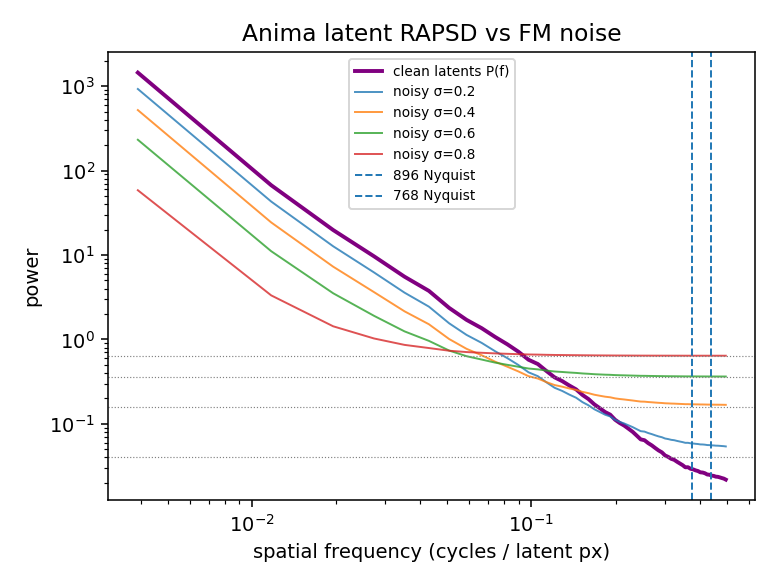
\includegraphics[width=\linewidth]{figs/rapsd_spectrum.png}
\caption{Latent RAPSD against the flow-matching noise floor at four
noise levels; dashed lines mark the demoted grids' Nyquist cuts.}
\label{fig:rapsd}
\end{subfigure}\hfill
\begin{subfigure}[t]{0.49\textwidth}
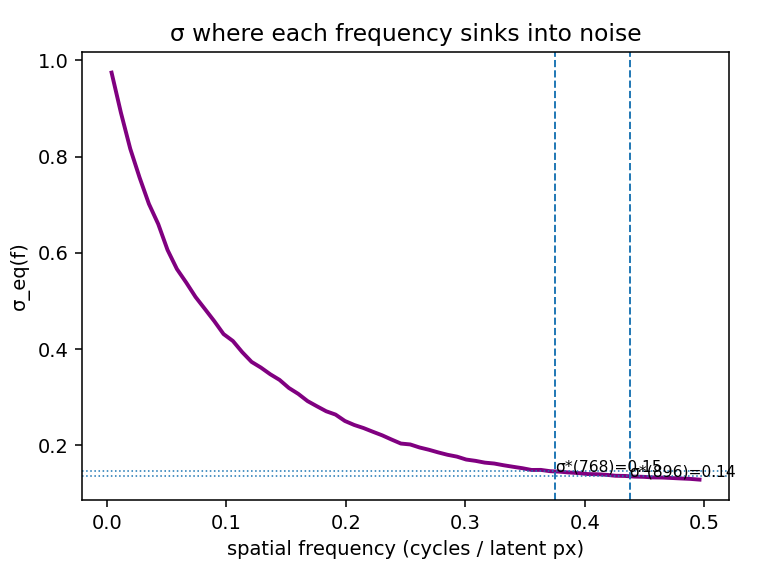
\includegraphics[width=\linewidth]{figs/rapsd_crossover.png}
\caption{The equal-power slice $\sigma_{\mathrm{eq}}(f)$ of the spectral
family. Predicted $\sigmastar$: $0.136$ / $0.146$ / ${\sim}0.20$ for
demotion to 896 / 768 / 512.}
\label{fig:sigmaeq}
\end{subfigure}
\caption{The spectral account, computed from the measured RAPSD and
transported to the training question (\S\ref{sec:spectral}): safety
would be predicted from $\sigma \approx 0.14$. Against the measurement
(Fig.~\ref{fig:verdict}) no tolerance reproduces the pattern
(Table~\ref{tab:null}): the equal-power crossover is off by
${\sim}3.5\times$, and the $2\times$ downscale, predicted safe by every
tolerance, certifies at no noise level.}
\label{fig:spectrum}
\end{figure}

\begin{figure}[t]
\centering
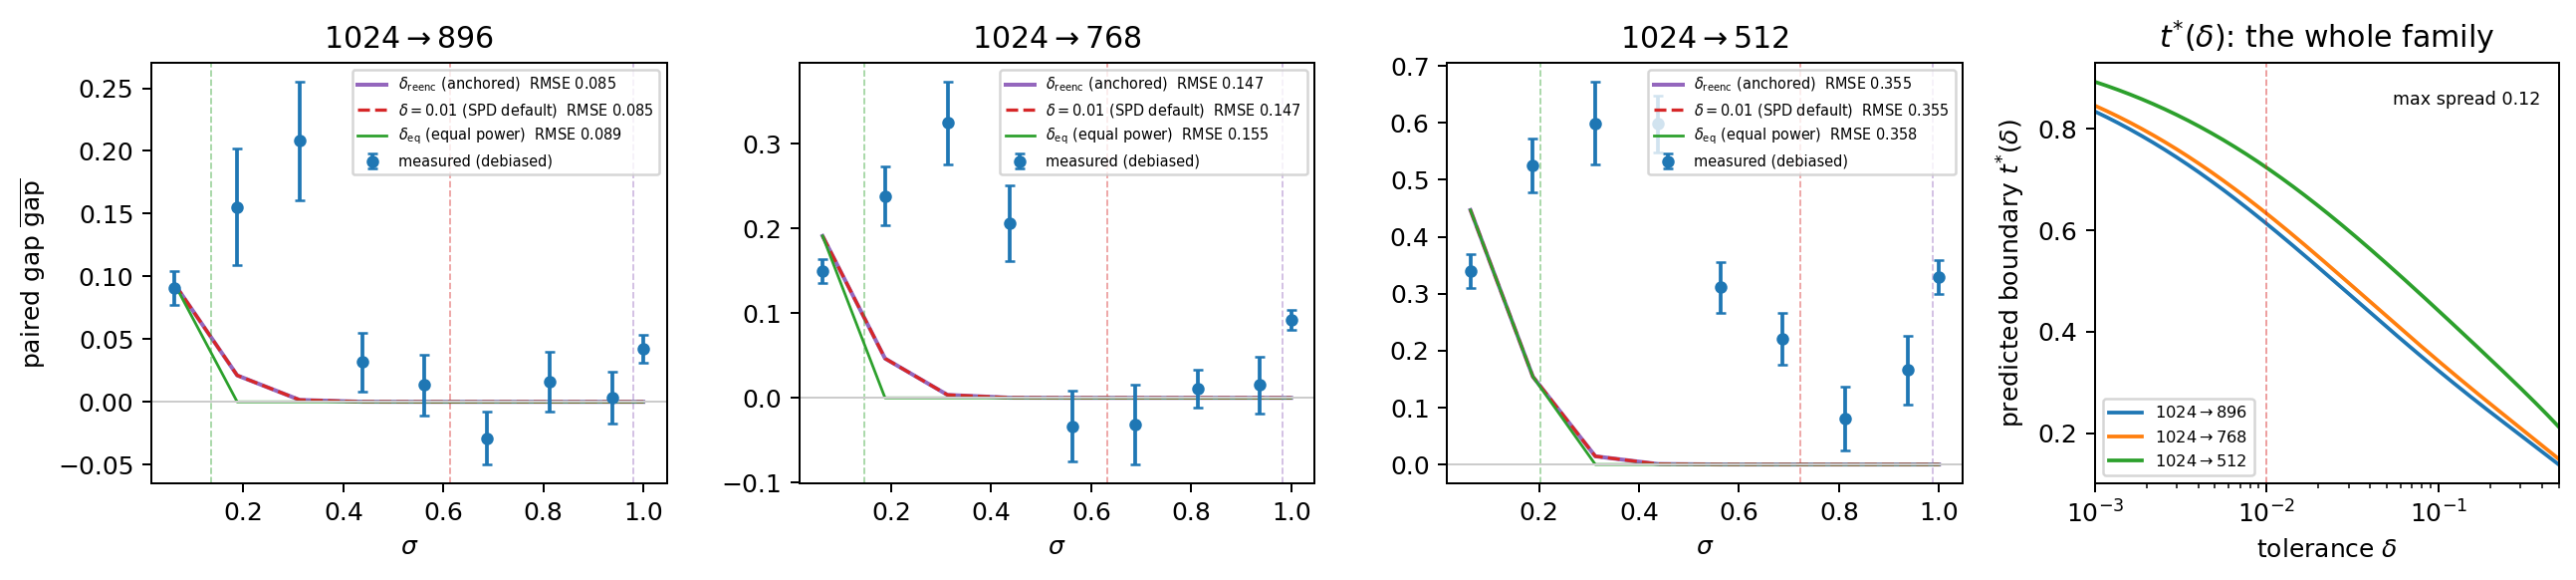
\includegraphics[width=\linewidth]{figs/e83_overlay.png}
\caption{The \emph{whole} tolerance family against the measurement:
the detail behind the single red curve of Fig.~\ref{fig:accounts}. Left
three panels: the measured debiased gap curves against the spectral
account transported through our bridge (the diagonal model's
destroyed-band mean-residual mismatch on the measured spectrum, through
the measured $\|\bar g_{\src}(\sigma)\|$ with a single gain calibrated
on the one safe route and no floor, which the family cannot express),
gated at $t^{*}(\delta)$ (dashed verticals) for the equal-power slice,
SPD's default $\delta = 0.01$, and the measured anchor
$\delta_{\reenc}$. The transported curve dies by $\sigma \approx 0.35$
on every route, so the two larger gates ($0.61$--$0.72$ and
$0.98$--$0.99$) act on an already-zero curve and coincide exactly;
the equal-power gate ($0.14$--$0.20$) is the only one that truncates
live curve, and it moves RMSE by at most $0.008$. All three therefore
land within $0.01$ of each other: $\delta$ is inert at the curve
level. Right: the boundary family $t^{*}(\delta)$; maximum route spread
$0.125$ in $\sigma$ over $\delta \in [10^{-3}, 0.5]$.}
\label{fig:e83}
\end{figure}

The tolerance $\delta$ of Eq.~\ref{eq:spd} is the account's one free
parameter, and this appendix instantiates the whole family. The choice
$\delta = (1+P_\omega)/2$ recovers the often-quoted equal-power
(input-SNR) crossover
$\sigma_{\mathrm{eq}} = \sqrt{P_\omega}/(1+\sqrt{P_\omega})$ as one
slice; \citet{xiao2026spd} ship an inference-side default
$\delta = 0.01$; and our own pipeline fixes a zero-free-parameter
anchor $\delta_{\reenc}$ by construction (below).

Table~\ref{tab:null} evaluates Eq.~\ref{eq:spd} at the demoted grids'
Nyquist frequencies $f_{\mathrm{cut}} = \tfrac{1}{2}\,e/e_0$ on the
$N{=}40$ mean radially-averaged latent power spectrum ($64$ radial
bins; $P$ at the $896/768/512$ cuts $= 0.025/0.029/0.065$;
Fig.~\ref{fig:spectrum}). Across
$\delta \in [0.001, 0.5]$ the mildest--harshest spread remains below
$0.13$, and the $1024{\to}896$ versus $896{\to}768$ boundaries (cut
frequencies $0.4375$ vs $0.4286$) separate by no more than $0.01$.
The parameter-free anchor $\delta_{\reenc}$ of \S\ref{sec:specscored} is
measured by the same estimator: RAPSD of the re-encode arm's latent error
(fresh resize--encode minus cached latent, the gradient probe's own
control chain) on the same probe set, interpolated at each route's cut
frequency. Measured ($N{=}40$, $64$ radial bins): error variance
$2.7\times10^{-5}$ against latent variance $0.419$;
$D(f_{\mathrm{cut}}) \approx 1.0\times10^{-5}$ at all three cuts
(p10--p90 over images within $[1, 2]\times10^{-5}$; per-band SNR
$P(f_{\mathrm{cut}})/D(f_{\mathrm{cut}}) \approx 2.5$--$4.4\times10^{3}$),
giving $t^{*}_{\reenc} = 0.98 / 0.98 / 0.99$ for $896/768/512$.

\paragraph{The ``wrong $\delta$'' objection, closed by construction.}
One might object that the right $\delta$ has simply not been chosen:
SPD's is an inference-side value selected on a speed--quality Pareto
ablation over generated images \citep{xiao2026spd}, and nothing ties it
to gradients. Our setting fixes one \emph{by construction}. The
demotion recipe pays a resize--VAE-encode round trip whose latent error
has measurable per-band power $D(f)$, expressed in exactly
Eq.~\ref{eq:spd}'s units, so $\delta_{\reenc}(e) :=
D(f_{\mathrm{cut}}(e))$ anchors the family with zero free parameters.
Measured (above), that anchor is tiny and image-generic, and the
boundary moves it forces are measured in Table~\ref{tab:null} and
Fig.~\ref{fig:e83}: every boundary is pushed to $t^{*} \approx 0.98$,
maximally conservative, and still structurally wrong in both
directions at once: it moves all three boundaries together (spread
$< 0.01$), certifies the measured-safe route only above
$\sigma \approx 0.98$ where the measurement certifies it from $0.5$,
and, like every member of the family, predicts the $2\times$ downscale
eventually safe when no noise level is. The confrontation of
\S\ref{sec:specscored} therefore does not hinge on the choice of
tolerance: the structural failures of \S\ref{sec:spectral}(a--c) are
$\delta$-independent at the boundary level, and $\delta$ is inert
outright at the curve level (Fig.~\ref{fig:e83}).

\section{Controlled-adapter replication of the verdict map}
\label{app:e7}

\begin{figure}[t]
\centering
\begin{subfigure}[t]{0.49\textwidth}
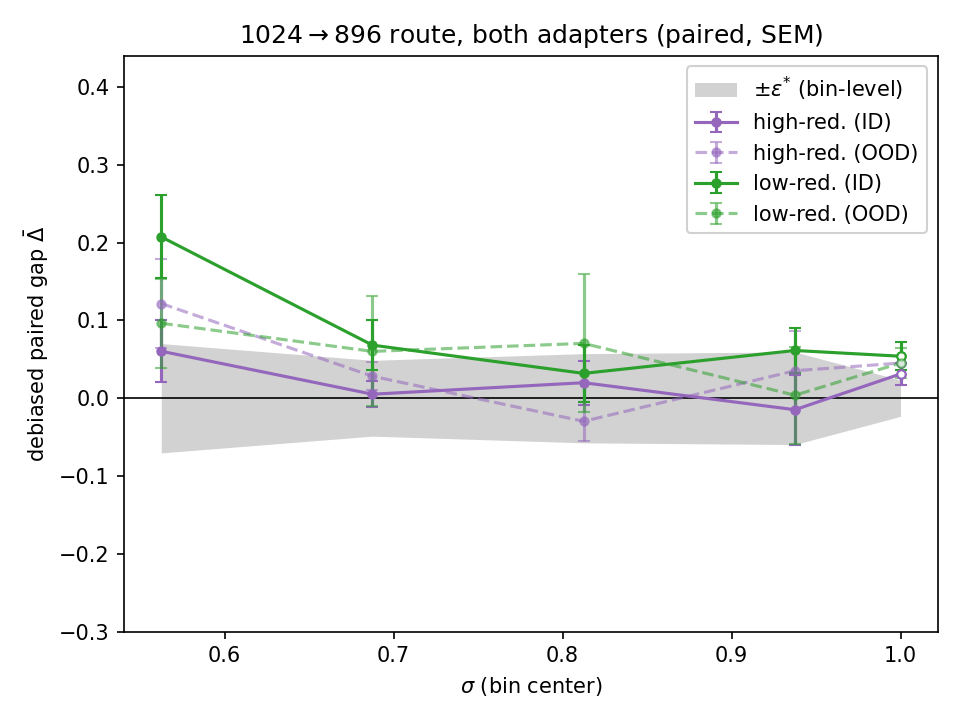
\includegraphics[width=\linewidth]{figs/gap_debiased_e7_route896.png}
\caption{$1024{\to}896$ (the certified route).}
\label{fig:e7route896}
\end{subfigure}\hfill
\begin{subfigure}[t]{0.49\textwidth}
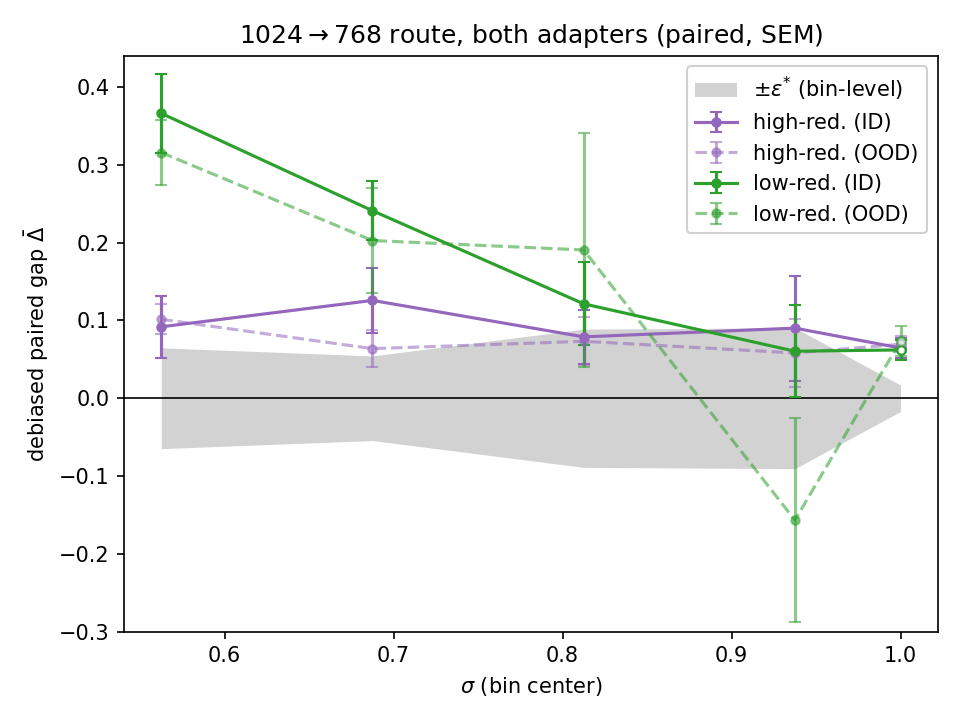
\includegraphics[width=\linewidth]{figs/gap_debiased_e7_route768.png}
\caption{$1024{\to}768$.}
\label{fig:e7route768}
\end{subfigure}
\caption{The Fig.~\ref{fig:gapcurves} recipe repeated on two controlled
adapters trained on opposite style clusters, one panel per route
($N{=}48$ stems per adapter, $D{=}8$/bin, high-$\sigma$ window; same
paired debiased estimator and trim; open markers the $\sigma{=}1$
endpoint bin; axes shared across panels). Unlike the main-text figures,
color encodes the \emph{adapter} (high- vs low-redundancy cluster);
solid curves are in-distribution stems, the adapter's own style
cluster ($n{=}36$: trained-on, held-out, and unseen-artist cells),
and dashed curves are out-of-distribution stems from the opposite
cluster ($n{=}12$). Gray band: bin-level $\pm\epsstar$ per
Eq.~\ref{eq:safe}, median of the two runs' full-$N$ SEMs for the
panel's route. The map replicates: on the certified route all four
adapter$\times$distribution curves reach the band inside the window,
on $768$ all four sit above it until the top, and within each panel the
dashed OOD curves track their solid ID counterparts.}
\label{fig:e7maps}
\end{figure}

The one-adapter limitation of \S\ref{sec:limitations} pre-registered a
controlled $2{\times}2$ factorial: two plain-LoRA checkpoints trained
under the original probe adapter's frozen recipe on opposite style
clusters (the top and bottom $12$ artists by median latent
redundancy, hereafter the high-redundancy, visually flat, and
low-redundancy, heavily textured, clusters), with stem-level
membership manifests frozen
before training ($124$ training images each, identical seeds). Each
adapter was probed on $48$ stems spanning four membership cells
($N{=}12$ each): trained-on, held-out images of trained artists,
unseen artists of the same cluster, and unseen artists of the
opposite cluster, with the cross-cluster stems shared between the two
runs so cross-adapter contrasts read paired per stem.
Figure~\ref{fig:e7maps} repeats the verdict-map recipe per route,
overlaying both adapters.

Three reads, stated at the bin-mean level (per-cell tables reproduce
from the archived per-image rows). First, the $(\text{route}, \sigma)$
shape replicates on both checkpoints (Fig.~\ref{fig:e7maps}). Second,
the factorial contrasts are null at instrument resolution: the
probe-style main effect and the adapter$\times$probe-style interaction
(the pre-registered verdict quantity) are both bounded below the
resolvable bin-mean effect (raw-gap paired interaction
$-0.022 \pm 0.027$ at $896$, $-0.015 \pm 0.059$ at $768$), and the
membership contrast (trained-on versus held-out) does not replicate in
sign across the two adapters. The map is therefore adapter- and
content-agnostic on this model at our resolution, supporting a
calibrate-once-per-model reading. Third, the one quantity that is
\emph{not} checkpoint-invariant is the absolute redraw-floor level:
in-window floor cosines sit at ${\approx}0.73$ for the
high-redundancy-cluster adapter versus ${\approx}0.50$ for the
low-redundancy-cluster adapter, uniformly across all four membership
cells. The floor's level is a property of the checkpoint (its gradient
stochasticity), while the safety map built on top of it is not.

\section{Per-bin verdict numbers, and the historical record}
\label{app:tables}

Table~\ref{tab:debiasedmap} is the numerical form of
Fig.~\ref{fig:gapcurves}, the paper's verdict map, and
Table~\ref{tab:floor} the debiased floor reads that
\S\ref{sec:ourscored} scores the graph term on. The remaining tables
are the raw-estimator record: retained for continuity and for the reads
defended in \S\ref{sec:instrument} (one-signed bias; paired same-grid
contrasts), not cited as debiased evidence. Table~\ref{tab:phase0} is
the uncorrected counterpart of the verdict map on the original coarse
grid, and its last two rows are the coarse-grid estimator context
(Fig.~\ref{fig:estimator} plots the same two curves on the dense
verdict grid).

\begin{figure}[t]
\centering
\begin{subfigure}[t]{0.46\textwidth}
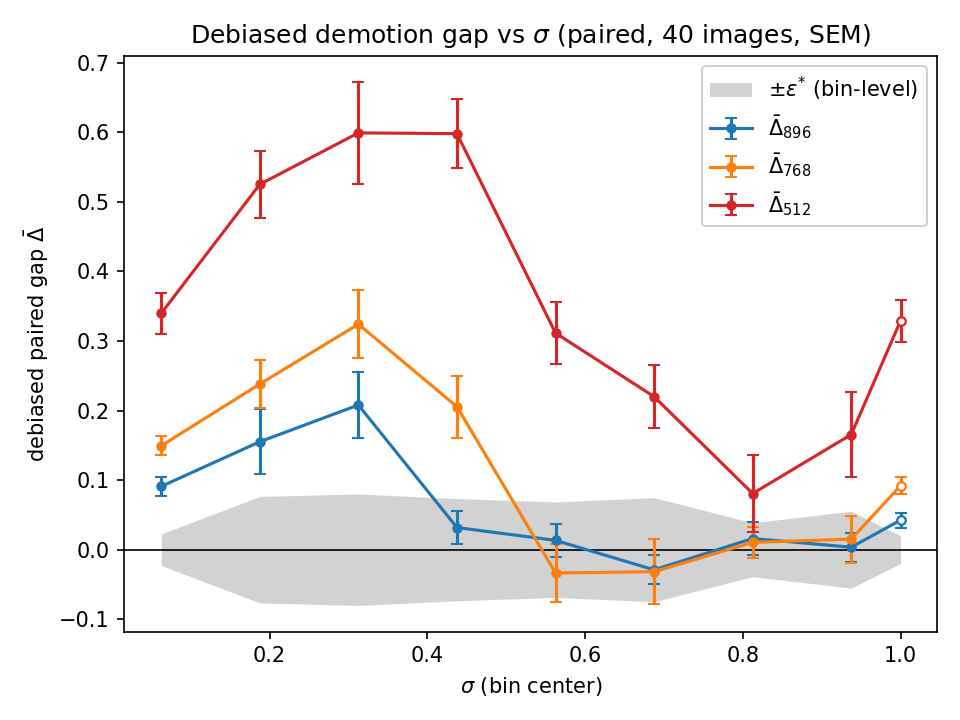
\includegraphics[width=\linewidth]{figs/gap_debiased.png}
\phantomcaption
\label{fig:gapcurves}
\end{subfigure}\hfill
\begin{subfigure}[t]{0.515\textwidth}
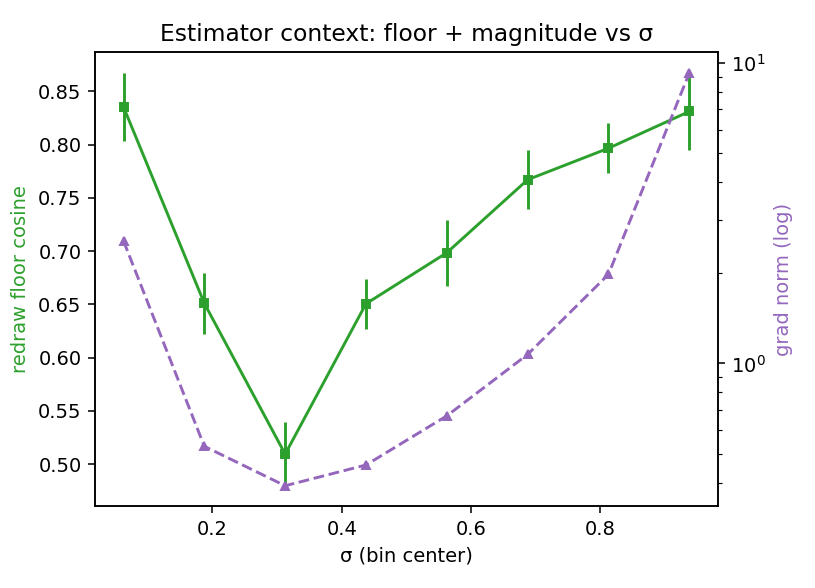
\includegraphics[width=\linewidth]{figs/estimator_context.png}
\phantomcaption
\label{fig:estimator}
\end{subfigure}
\caption{The measurement in detail.
(a)~Debiased demotion gap per $\sigma$-bin, all three routes on one
shared axis, paired against the re-encoding control ($1024$-tier
natives, $N{=}40$; per-bin values and
SEMs in Table~\ref{tab:debiasedmap}; gray band: bin-level
$\pm\epsstar$ (\S\ref{sec:instrument}); open markers: the $\sigma{=}1$
endpoint bin): safety is a per-route boundary. The $896$ route
enters the band at $\sigma \approx 0.5$, $768$ falls only to a
low-excess shelf ($+0.02$--$0.04$ over $0.65 < \sigma < 0.95$, short
of the strict margin), and $512$ never falls inside the band (closest
approach $+0.12 \pm 0.05$ at $\sigma = 0.96$); all three boundaries
stand against the spectral family's prediction of
$\sigma \approx 0.14$--$0.20$.
(b)~The estimator context those curves are read through: the
redraw-floor cosine and the U-shaped gradient norm
$\|\bar g_{\src}(\sigma)\|$.}
\label{fig:verdict}
\end{figure}

\begin{table}[h]
\caption{\textbf{Debiased verdict map} (plotted in
Fig.~\ref{fig:gapcurves}): paired per-image debiased excess
$\bgap$ (SEM) against the re-encoding control, $1024$-tier natives
($N{=}40$, $D{=}12$/bin, deterministic kernels, on a segmented grid
dense below $\sigma = 0.1$ and above $0.9$: $14$ interior bins plus
a $\sigma{=}1$ endpoint bin; trimmed per \S\ref{sec:instrument},
retaining $36$--$40$ images per cell). Bin-level $\epsstar$ at this
$(N, D)$ is $0.02$--$0.07$. A reconstruction check (the realized
excess rebuilt from per-arm means) flags the three $\sigma \le 0.06$
bins as partly estimator inflation, so the raw-paired excess is the
primary read there ($896$: $+.037/+.118/+.221$; $768$:
$+.065/+.202/+.275$; $512$: $+.172/+.406/+.497$), up to $0.08$
smaller with the same verdicts.}
\label{tab:debiasedmap}
\centering
\small
\begin{tabular}{cccc}
\toprule
$\sigma$ bin center & $1024{\to}896$ & $1024{\to}768$ & $1024{\to}512$ \\
\midrule
0.013 & $+.029$ {\scriptsize(.006)} & $+.059$ {\scriptsize(.012)} & $+.154$ {\scriptsize(.025)} \\
0.038 & $+.158$ {\scriptsize(.016)} & $+.219$ {\scriptsize(.026)} & $+.480$ {\scriptsize(.029)} \\
0.063 & $+.239$ {\scriptsize(.019)} & $+.323$ {\scriptsize(.028)} & $+.575$ {\scriptsize(.037)} \\
0.088 & $+.282$ {\scriptsize(.026)} & $+.366$ {\scriptsize(.024)} & $+.622$ {\scriptsize(.033)} \\
0.167 & $+.218$ {\scriptsize(.041)} & $+.348$ {\scriptsize(.033)} & $+.640$ {\scriptsize(.050)} \\
0.300 & $+.291$ {\scriptsize(.047)} & $+.378$ {\scriptsize(.038)} & $+.714$ {\scriptsize(.045)} \\
0.433 & $+.067$ {\scriptsize(.032)} & $+.253$ {\scriptsize(.041)} & $+.504$ {\scriptsize(.065)} \\
0.567 & $+.029$ {\scriptsize(.023)} & $+.078$ {\scriptsize(.019)} & $+.360$ {\scriptsize(.055)} \\
0.700 & $+.026$ {\scriptsize(.016)} & $+.032$ {\scriptsize(.023)} & $+.242$ {\scriptsize(.039)} \\
0.833 & $-.027$ {\scriptsize(.020)} & $+.034$ {\scriptsize(.023)} & $+.218$ {\scriptsize(.053)} \\
0.913 & $-.007$ {\scriptsize(.014)} & $+.039$ {\scriptsize(.013)} & $+.205$ {\scriptsize(.047)} \\
0.938 & $-.039$ {\scriptsize(.026)} & $+.019$ {\scriptsize(.019)} & $+.200$ {\scriptsize(.049)} \\
0.963 & $-.008$ {\scriptsize(.015)} & $+.026$ {\scriptsize(.016)} & $+.120$ {\scriptsize(.045)} \\
0.988 & $+.018$ {\scriptsize(.028)} & $+.034$ {\scriptsize(.045)} & $+.217$ {\scriptsize(.052)} \\
\midrule
1.0 (endpoint) & $+.034$ {\scriptsize(.011)} & $+.130$ {\scriptsize(.030)} & $+.406$ {\scriptsize(.049)} \\
\bottomrule
\end{tabular}
\end{table}

\begin{table}[h]
\caption{\textbf{The floor, debiased} (scored in
\S\ref{sec:ourscored}). \textbf{Endpoint}: at $\sigma{=}1$ the
input is exactly $\epsilon$ on every grid, so the input-mediated data
term vanishes by construction. \textbf{x-zero}: the image is removed
from input \emph{and} target; any surviving gap is pure graph-shape
sensitivity. Debiased draw-limit values $\dgap_\infty$ [bootstrap 95\%
CI over images] from nested draw sweeps (endpoint: $N{=}12$,
$D = 4 \ldots 64$; x-zero: $N{=}40$, $D = 4 \ldots 32$). The two
columns agree within CI at every route; our pre-registered kill switch
(all endpoint gaps ${\approx}\,0$) does not fire; and no member of the
spectral family can produce a nonzero entry here.}
\label{tab:floor}
\centering
\small
\begin{tabular}{lcc}
\toprule
route & endpoint $\dgap_\infty$ [95\% CI] &
x-zero $\dgap_\infty$ [95\% CI] \\
\midrule
native self-floor (cosine) & $1.005$ $[0.994, 1.016]$ & --- \\
re-encoding control & $-0.003$ $[-0.017, +0.008]$ & --- \\
$1024{\to}896$ & $+0.019$ $[+0.010, +0.030]$ & $+0.034$ $[+0.017, +0.058]$ \\
$1024{\to}768$ & $+0.056$ $[+0.043, +0.071]$ & $+0.074$ $[+0.053, +0.094]$ \\
$1024{\to}512$ & $+0.304$ $[+0.197, +0.424]$ & $+0.283$ $[+0.232, +0.332]$ \\
\bottomrule
\end{tabular}
\end{table}

\begin{table}[h]
\caption{\textbf{Raw estimator} (historical record; superseded by
Table~\ref{tab:debiasedmap}): demotion gap by
$\sigma$-bin, $1024$-tier natives ($N{=}40$,
bin-mean SEM ${\sim}0.02$, re-encoding control $|\gap_\reenc| \le 0.054$
everywhere, split-half reliability $0.73$--$0.83$). Bold = within the
re-encoding band. Raw values understate mid-$\sigma$ gaps (the floor
attenuates the read) and overstate endpoint floors (single-estimate
variance bias); the debiased map corrects both.}
\label{tab:phase0}
\centering
\small
\begin{tabular}{lcccccccc}
\toprule
$\sigma$ bin center & 0.06 & 0.19 & 0.31 & 0.44 & 0.56 & 0.69 & 0.81 & 0.94 \\
\midrule
$\gap_{896}$ (ratio $0.875$) & .110 & .162 & .148 & .137 & \textbf{.048} & \textbf{.030} & \textbf{.030} & .053 \\
$\gap_{768}$ (ratio $0.75$)  & .144 & .216 & .208 & .223 & .164 & .163 & .115 & .063 \\
$\gap_{512}$ (ratio $0.5$)   & .348 & .410 & .355 & .469 & .430 & .391 & .289 & .296 \\
\midrule
$\cos_{\mathrm{floor}}$ & .84 & .65 & .51 & .65 & .70 & .77 & .80 & .83 \\
$\|g\|$ (native) & 2.6 & 0.5 & 0.4 & 0.5 & 0.7 & 1.1 & 2.0 & 9.3 \\
\bottomrule
\end{tabular}
\end{table}

\begin{table}[h]
\caption{Raw endpoint reads ($D{=}16$, $N{=}40$) beside their debiased
draw-limit values (Table~\ref{tab:floor}), the debiasing's revision
record: the $768$ floor halves, the $896$ floor surfaces.}
\label{tab:rawendpoint}
\centering
\small
\begin{tabular}{lcc}
\toprule
route & raw endpoint ($D{=}16$) & endpoint $\dgap_\infty$ [95\% CI] \\
\midrule
native self-floor (cosine) & $0.85$ & $1.005$ $[0.994, 1.016]$ \\
re-encoding control & $-0.038$ & $-0.003$ $[-0.017, +0.008]$ \\
$1024{\to}896$ & $-0.009$ & $+0.019$ $[+0.010, +0.030]$ \\
$1024{\to}768$ & $+0.127$ & $+0.056$ $[+0.043, +0.071]$ \\
$1024{\to}512$ & $+0.326$ & $+0.304$ $[+0.197, +0.424]$ \\
\bottomrule
\end{tabular}
\end{table}

\begin{table}[h]
\caption{Iso-severity probe (\textbf{raw estimator}): gap by $\sigma$-bin
on the $1280$-tier cache
($N{=}24$, $4$ draws/bin) against the corpus $1024{\to}896$ curve. The
ratio-matched routes coincide within ${\sim}1.4$ combined SEM at every bin
despite a $1.6\times$ difference in absolute target size; the same-native
harsher-ratio route separates. $^{*}$$896$'s canonical $16$-draw endpoint
is $-0.009$ raw, $+0.019$ debiased (Table~\ref{tab:floor}).}
\label{tab:isoseverity}
\centering
\small
\begin{tabular}{lccccc}
\toprule
$\sigma$ & 0.125 & 0.375 & 0.625 & 0.875 & 1.0 \\
\midrule
re-encoding control & $+.047$ & $-.005$ & $+.048$ & $+.020$ & $-.012$ \\
$1280{\to}1120$ (ratio $.875$) & .129 & .110 & .054 & $-.012$ & $-.007$ \\
$1280{\to}1024$ (ratio $.80$)  & .170 & .178 & .111 & .002 & .061 \\
$1024{\to}896$ (ratio $.875$)  & .132 & .076 & .077 & .049 & .100$^{*}$ \\
\bottomrule
\end{tabular}
\end{table}

\begin{table}[h]
\caption{Ratio-transfer run (\textbf{raw estimator}): $896$-tier natives
($N{=}40$), pre-registered
bar ``$\gap_{768}$ within the re-encoding band at $\sigma \ge 0.5$'':
\textbf{fails} (residual $0.06$--$0.12$, ${\sim}2\times$ the
$1024{\to}896$ plateau; ${\sim}$half of it is expected estimator bias,
\S\ref{sec:instrument}; the separation is independently confirmed by
the debiased same-grid floors, \S\ref{sec:ourscored}).}
\label{tab:phase1a}
\centering
\small
\begin{tabular}{lcccccccc}
\toprule
$\sigma$ bin & 0.06 & 0.19 & 0.31 & 0.44 & 0.56 & 0.69 & 0.81 & 0.94 \\
\midrule
$896{\to}768$ & .114 & .209 & .168 & .143 & .124 & .056 & .092 & .061 \\
$896{\to}512$ & .318 & .372 & .308 & .340 & .320 & .280 & .329 & .217 \\
\bottomrule
\end{tabular}
\end{table}

\begin{table}[h]
\caption{Route-uniformity (in amplitude) of the mean prediction
residual: cross-grid
excess of $\bar r = \mathbb{E}_\epsilon[\hat v - (\epsilon - x)]$ over
split-half floors (relative $L_2$; same-grid re-encoding control
$\le 0.02$ everywhere). The three main routes coincide within
${\sim}\pm 0.02$ at every $\sigma$ while their gradient floors span $0$ to
$0.3$. This is a norm read; the direction-resolved follow-up
(Appendix~\ref{app:instrument}) shows the underlying mismatch directions
are image- and route-specific.}
\label{tab:residual}
\centering
\small
\begin{tabular}{lccccc}
\toprule
$\sigma$ & 0.125 & 0.375 & 0.625 & 0.875 & 1.0 \\
\midrule
$1280{\to}1024$ & .885 & .825 & .715 & .465 & .360 \\
$1024{\to}896$  & .862 & .808 & .706 & .459 & .378 \\
$896{\to}768$   & .860 & .814 & .715 & .466 & .393 \\
$768{\to}512$   & .897 & .872 & .767 & .508 & .435 \\
\bottomrule
\end{tabular}
\end{table}

\begin{table}[h]
\caption{Depth localization of the floor (\textbf{raw estimator}): mean
per-block gap at
$\sigma{=}1$, early $=$ blocks 0--9, late $=$ 14--27, for the endpoint
(ep) and x-zero (xz) probes. Early blocks carry ${\sim}3\times$ the
late-block gap. The apparent content share (ep $-$ xz) is a late-block
minority effect in raw units; the debiased draw-limit comparison finds
ep $=$ xz within CI at the whole-adapter level
(Table~\ref{tab:floor}). Within a block every module type sits in
$0.22$--$0.31$ at $512/\sigma{=}1$, including the query and key rows of
the fused QKV projection: landing-side uniformity, which is why the
positional share needed an origin-side intervention to find.}
\label{tab:depth}
\centering
\small
\begin{tabular}{lcccc}
\toprule
route & ep early & ep late & xz early & xz late \\
\midrule
$1024{\to}512$ & .357 & .223 & .351 & .125 \\
$1024{\to}768$ & .164 & .085 & .121 & .033 \\
$1024{\to}896$ & .023 & .015 & .044 & .012 \\
\bottomrule
\end{tabular}
\end{table}

\begin{table}[h]
\caption{Positional-interpolation intervention at the $\sigma{=}1$
endpoint ($N{=}40$, $16$ draws; \textbf{raw} arm values; the paired
$\Delta$ column is a same-grid contrast in which the finite-draw bias
cancels to first order): exact phase-geometry alignment erases the
mild-route floor and ${\sim}30\%$ of the harsh-route floor.}
\label{tab:pi}
\centering
\small
\begin{tabular}{lcccc}
\toprule
route & plain (SEM) & PI-aligned (SEM) & paired $\Delta$ (SEM) & improved \\
\midrule
$1024{\to}896$ (control) & $-0.021$ (.041) & $-0.040$ (.040) & --- & --- \\
$1024{\to}768$ & $+0.080$ (.048) & $-0.001$ (.039) & $+0.081$ (.031) & $78\%$ \\
$1024{\to}512$ & $+0.320$ (.058) & $+0.224$ (.056) & $+0.096$ (.039) & $70\%$ \\
\bottomrule
\end{tabular}
\end{table}
